This section is a brief introduction to networks from its basic structure to the chosen one by us.
Basically is a telecommunications network that allows computers to exchange data. That permit to coordinate and share resources between to and fro devices in order to cooperate and achieve a common objective. 

Every computer has a number of connections, among wired or wireless channels, to the other devices that exists in the network. Information travel by these channels in form of packets codified under many kinds of protocols. 

Every connection and the form of the packets depend on the mentioned protocols. In this project we consider only two: TCP and UDP protocols.

\begin{itemize}
	\item TCP is a connection oriented stream over an IP network. It guarantees that all sent packets will reach the destination in the correct order. This imply the use of acknowledgment packets sent back to the sender, and automatic retransmission, causing additional delays and a general less efficient transmission than UDP.

	\item UDP a is connection-less protocol. Communication is datagram oriented. The integrity is guaranteed only on the single datagram. Datagrams reach destination and can arrive out of order or don't arrive at all. It is more efficient than TCP because it uses non ACK. It's generally used for real time communication, where a little percentage of packet loss rate is preferable to the overhead of a TCP connection.
\end{itemize}

%----------------------------------------------------------------
\subsection{Hardware}
\begin{wrapfigure}{r}{0.5\textwidth}
	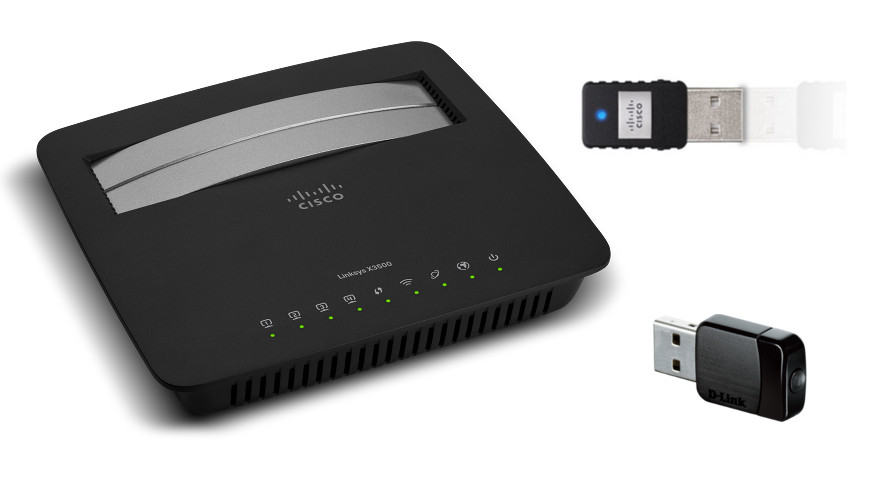
\includegraphics[width=0.5\textwidth]{../Images/c2/hardware_comm.jpg}
	\caption{WiFi PA and USB adapters}
	\label{fig:hardwareComm}
\end{wrapfigure}

This section briefly describes the architecture of communication. In order to be versatile and flexible, the experiments will use one router and one WiFi adapter per quadrotor. We talk about flexibility because with those devices don't restrict the software, i. e., the whole system can bee exchanged with GSM modules and cloud computation or inside a computer with simulated targets and persecutors (Quadrotors).

%----------------------------------------------------------------
\subsection{Software, protocol and messages}

\begin{wrapfigure}{r}{0.5\textwidth}
	\begin{center}
		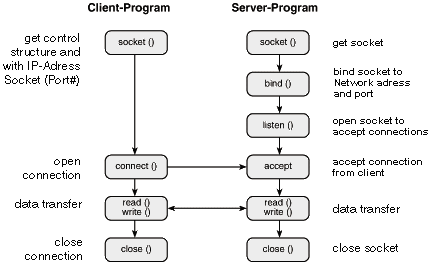
\includegraphics[width=0.5\textwidth, natwidth=448, natheight=263]{../Images/c2/socketstcpip.png}
	\end{center}
	\caption{Sockets and TCP-IP}
	\label{fig:socketstcpip}
\end{wrapfigure}

To communicate between devices every application (or program) use a sockets \cite{SocketWiki}. Particularly, an implementation developed initially for this project that can be found in BOViL \cite{BOViL}. Sockets are configured with the TCP/IP protocol \cite{TCPIP}. \\


